\documentclass{standalone}
\usepackage{tikz}
\usepackage{amsmath}
\usetikzlibrary{positioning, shapes.geometric, arrows}

\tikzset{
    conv/.style={rectangle, draw=red, fill=red!20, minimum width=1cm, minimum height=1cm},
    dense/.style={circle, draw=blue, fill=blue!20, minimum size=0.5cm},
    pooling/.style={rectangle, draw=cyan, fill=cyan!20, minimum width=1cm, minimum height=1cm},
    flatten/.style={rectangle, draw=black, minimum width=0.8cm, minimum height=2cm},
    arrow/.style={->, thick}
}

\begin{document}

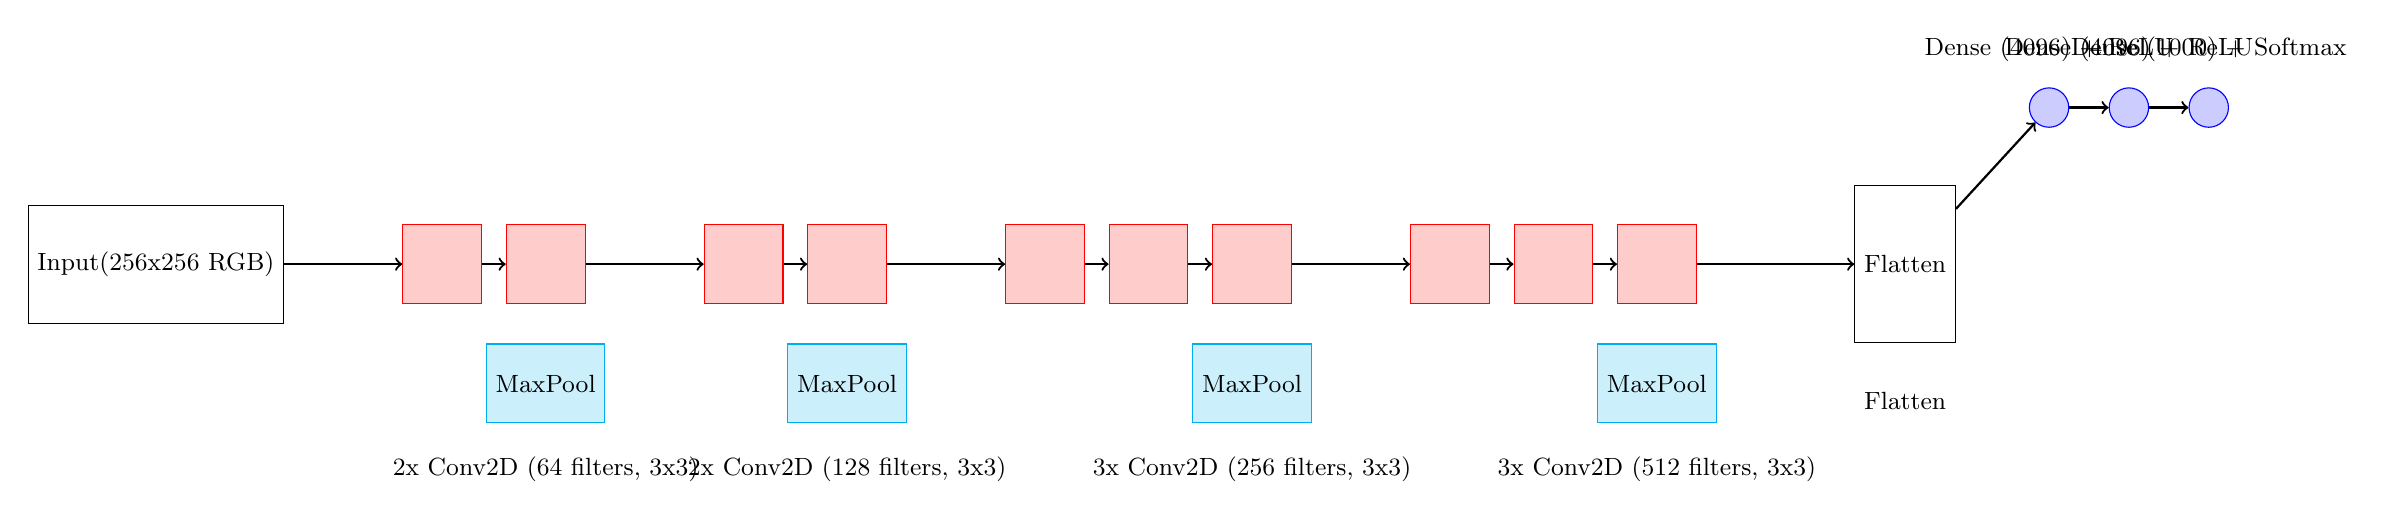
\begin{tikzpicture}[node distance=1.5cm, every node/.style={font=\small}]

% Input image
\node (input) [rectangle, draw, minimum width=1.5cm, minimum height=1.5cm] {Input\\(256x256 RGB)};

% First conv block
\node (conv1a) [conv, right=of input] {};
\node (conv1b) [conv, right=0.3cm of conv1a] {};
\node (pool1) [pooling, below=0.5cm of conv1b] {MaxPool};

% Second conv block
\node (conv2a) [conv, right=1.5cm of conv1b] {};
\node (conv2b) [conv, right=0.3cm of conv2a] {};
\node (pool2) [pooling, below=0.5cm of conv2b] {MaxPool};

% Third conv block
\node (conv3a) [conv, right=1.5cm of conv2b] {};
\node (conv3b) [conv, right=0.3cm of conv3a] {};
\node (conv3c) [conv, right=0.3cm of conv3b] {};
\node (pool3) [pooling, below=0.5cm of conv3c] {MaxPool};

% Fourth conv block
\node (conv4a) [conv, right=1.5cm of conv3c] {};
\node (conv4b) [conv, right=0.3cm of conv4a] {};
\node (conv4c) [conv, right=0.3cm of conv4b] {};
\node (pool4) [pooling, below=0.5cm of conv4c] {MaxPool};

% Flatten
\node (flatten) [flatten, right=2cm of conv4c] {Flatten};

% Dense layers
\node (dense1) [dense, above right=0.8cm and 1cm of flatten] {};
\node (dense2) [dense, right=0.5cm of dense1] {};
\node (dense3) [dense, right=0.5cm of dense2] {};

% Arrows between layers
\draw[arrow] (input) -- (conv1a);
\draw[arrow] (conv1a) -- (conv1b);
\draw[arrow] (conv1b) -- (conv2a);
\draw[arrow] (conv2a) -- (conv2b);
\draw[arrow] (conv2b) -- (conv3a);
\draw[arrow] (conv3a) -- (conv3b);
\draw[arrow] (conv3b) -- (conv3c);
\draw[arrow] (conv3c) -- (conv4a);
\draw[arrow] (conv4a) -- (conv4b);
\draw[arrow] (conv4b) -- (conv4c);
\draw[arrow] (conv4c) -- (flatten);
\draw[arrow] (flatten) -- (dense1);
\draw[arrow] (dense1) -- (dense2);
\draw[arrow] (dense2) -- (dense3);

% Labels
\node[below=0.3cm of pool1] {2x Conv2D (64 filters, 3x3)};
\node[below=0.3cm of pool2] {2x Conv2D (128 filters, 3x3)};
\node[below=0.3cm of pool3] {3x Conv2D (256 filters, 3x3)};
\node[below=0.3cm of pool4] {3x Conv2D (512 filters, 3x3)};

\node[below=0.5cm of flatten] {Flatten};
\node[above=0.2cm of dense1] {Dense (4096) + ReLU};
\node[above=0.2cm of dense2] {Dense (4096) + ReLU};
\node[above=0.2cm of dense3] {Dense (1000) + Softmax};

\end{tikzpicture}

\end{document}